The application designed and implemented in parallell with this report is a proof-of-concept of an application used for construction. The application is intended to function as a substitute for instruction manuals, where Google Glass will allow the user to scroll through instructions hands-free. A proof-of-concept of a similar application for smartphones has been designed and implemented as well, in order to provide a point of reference as well as help evaluate the pros and cons of using Google Glass.

As seen in Figure~\ref{cardDesign}, the application is designed as a slide view, with only one slide being displayed at a time. The instructions are to be divided into several steps, each presented on separate slides which users may scroll through at their own pace. On Google Glass, users may scroll through the application using voice commands in order to make the application truly hands-free. By applying the slide view design users may focus on one instruction at a time. Also, the amount of information presented on screen at the same time is also minimised depending on the limitations of the specific device.
%The application is meant to scan a QR Code, which will give information on the product, enabling the application to retrieve building instructions from a back end database. The instructions, as well as necessary components, will then be presented on screen in a slide show, giving users the ability to scroll through at their own pace.

	\begin{figure}[ht!]
		\centering
		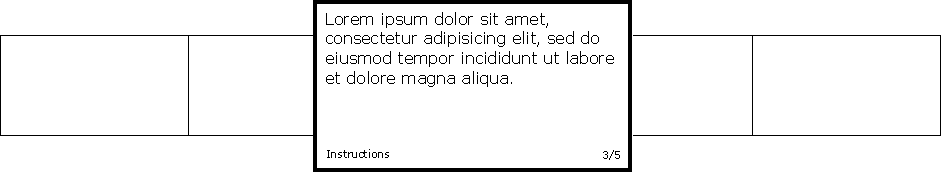
\includegraphics[width=150mm]{images/cardDesign2}
		\caption{A simple sketch of the application's GUI design.}
		\label{cardDesign}
	\end{figure}

The instructions are to be the major focus of each slide, with the instruction covering most of the slide. At the bottom additional information may be found, such as a label which, for instance, specifies that the information being presented on the current slide is an instruction (other information may also be presented, such as components necessary in order to complete the instructions). The design has been heavily inspired by Google's own guidelines as to how applications for Google Glass should be designed.
%	\begin{figure}[ht!]
%		\centering
%   	\subfloat[The Google Glass application.]{{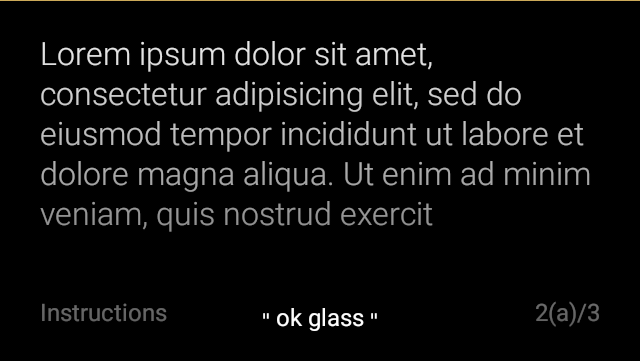
\includegraphics[width=70mm]{images/googleGlassAppScreenshot} }}
%  	 \qquad
%   	\subfloat[The smartphone application.]{{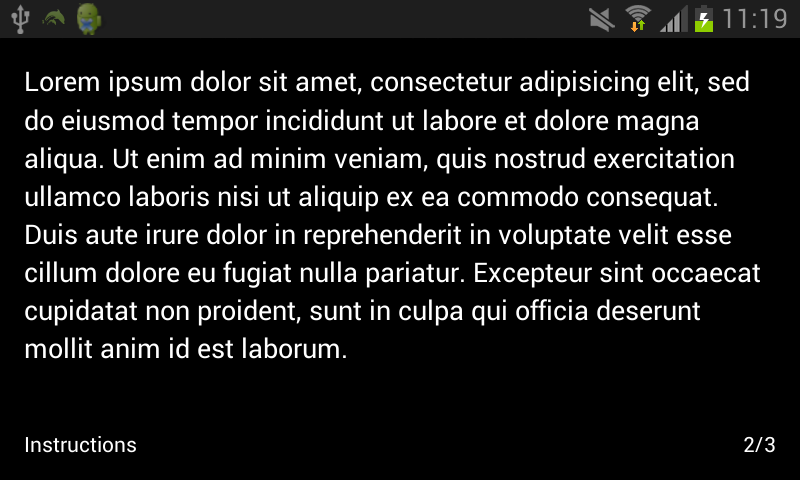
\includegraphics[width=70mm]{images/smartphoneAppScreenshot} }}
%   	\qquad
%		\caption{TODO}
%		\label{applicationScreenshot}
%	\end{figure}

\subsubsection{Glassware Flow Designer}
Google provides developers with a design tool to help them visualise applications prior to implementation. The design tool, called ``Glassware Flow Designer''~\cite{glasswareFlowDesigner}, allows developers to discover recommended design patterns and to see the flow of their application prior to implementation.

In Figure~\ref{glassFlowDesign} the Glass Flow Design for the Google Glass application described in this report is shown. When the application launches the user is supposed to scan a QR code. After successfully doing so the product name will be displayed, in order to help the user confirm that the correct instructions have been loaded in. Next are slides which shows necessary components. After components comes instructions. The slides can be controlled either through swiping on the Google Glass touchpad or through voice commands.

	\begin{figure}[ht!]
		\centering
		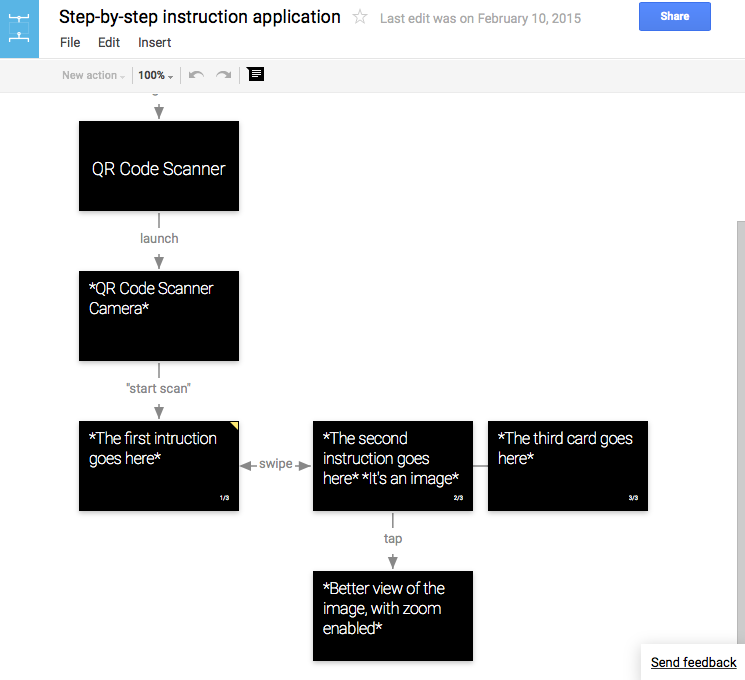
\includegraphics[width=150mm]{images/glaswareFlowDesignerScreenshot}
		\caption{Glass Flow Design of the Google Glass application.}
		\label{glassFlowDesign}
	\end{figure}